\documentclass[tikz,border=4pt]{standalone}
\usepackage{pgfplots}
\pgfplotsset{compat=1.18}
\usepgfplotslibrary{groupplots}
\begin{document}
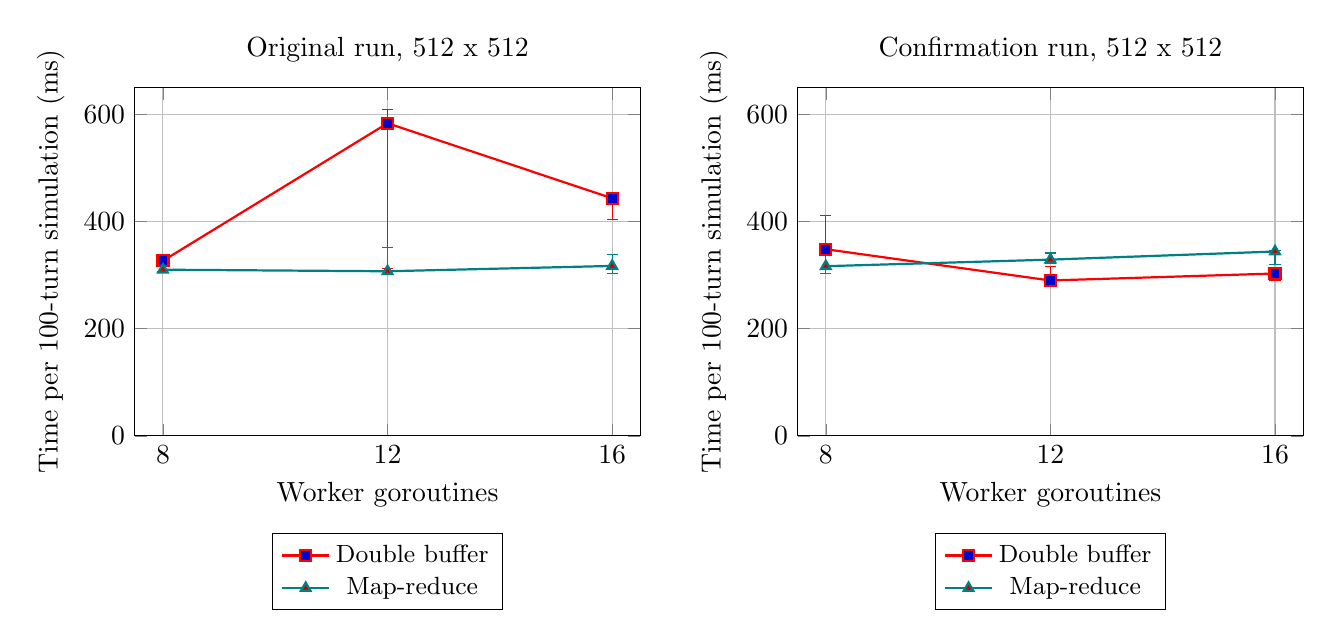
\begin{tikzpicture}
\begin{groupplot}[group style={group size=2 by 1,horizontal sep=20mm},
width=8cm,height=6cm,xlabel={Worker goroutines},
ylabel={Time per 100-turn simulation (ms)},
xtick={8,12,16},xmin=7.5,xmax=16.5,ymin=0,ymax=650,grid=major,
legend style={font=\small,at={(0.5,-0.28)},anchor=north}]
\nextgroupplot[title={Original run, 512 x 512}]
\addplot+[color=red,mark=square*,thick,error bars/.cd,y dir=both,y explicit] coordinates {(8,326.902948) += (0,6.738007) -= (0,8.519483) (12,583.937138) += (0,25.967888) -= (0,271.108592) (16,443.703939) += (0,1.526141) -= (0,39.831378)};
\addlegendentry{Double buffer}
\addplot+[color=teal,mark=triangle*,thick,error bars/.cd,y dir=both,y explicit] coordinates {(8,310.286925) += (0,24.927749) -= (0,3.861770) (12,307.357640) += (0,43.783080) -= (0,1.027182) (16,317.336201) += (0,20.900251) -= (0,13.973511)};
\addlegendentry{Map-reduce}
\nextgroupplot[title={Confirmation run, 512 x 512}]
\addplot+[color=red,mark=square*,thick,error bars/.cd,y dir=both,y explicit] coordinates {(8,348.532631) += (0,63.610970) -= (0,35.256529) (12,290.138523) += (0,26.421978) -= (0,1.904575) (16,303.173777) += (0,7.182159) -= (0,12.312776)};
\addlegendentry{Double buffer}
\addplot+[color=teal,mark=triangle*,thick,error bars/.cd,y dir=both,y explicit] coordinates {(8,316.826814) += (0,29.813904) -= (0,14.425070) (12,329.107674) += (0,12.450623) -= (0,6.524010) (16,344.257648) += (0,2.614107) -= (0,24.539117)};
\addlegendentry{Map-reduce}
\end{groupplot}
\end{tikzpicture}
\end{document}
